\documentclass[11pt,letterpaper]{article}
\usepackage[utf8]{inputenc}

%----- Configuración del estilo del documento------%
\usepackage{epsfig,graphicx}
\usepackage[left=2cm,right=2cm,top=1.8cm,bottom=2.3cm]{geometry}
\usepackage{fancyhdr}
\usepackage{lastpage}
\pagestyle{fancy}
\fancyhf{}

\usepackage{amsmath,amsthm,amssymb, tikz}
\usepackage{graphicx}
%%Use this package for matrices
\usepackage{array}
\usepackage{breqn}
\usepackage{multicol}
\usepackage{lipsum}
\usepackage{caption}
\usepackage{subcaption}
\usepackage{booktabs}

%%%%%%%%%%%%%%%%%%%%%%%%%%%%%%%%%%%%%%%%%%%%%%%%%%%%%%%%%%%%%%%%%%%%%%%%%%%%%%%%
\usepackage{amsmath}
\usepackage{amssymb}
\usepackage{amsthm}
\usepackage{float}
\usepackage[export]{adjustbox}

%%%%%%%%%%%%%%%%%%%%%%%%%%%%%%%%%%%%%%%%%%%%%%%%%%%%%%%%%%%%%%%%%%%%%%%%%%%%%%%%

\usepackage{lipsum}



\begin{document}

%%%%%%%%%%%%%%%%%%%%%%%%%%%%%%%%%%%%%%%%%%%%%%%%%%%%%%%%%%%%%%%%%%%%%%%%%%%%%%%%

\begin{center}
    \begin{minipage}{10cm}
    	\begin{center}
    	\textbf{\large Project 4}\\[0.1cm]
        \textbf{Inesh Chakrabarti, Lawrence Liu, Nathan Wei}\\[0.1cm]
    	\end{center}
    \end{minipage}\hfill
\end{center}

\rule{17cm}{0.1mm}

%%%%%%%%%%%%%%%%%%%%%%%%%%%%%%%%%%%%%%%%%%%%%%%%%%%%%%%%%%%%%%%%%%%%%%%%%%%%%%%%

\section*{Introduction}
For the first part of this project we will do regression analysis. The dataset 
we chose to use is one of diamond characteristics. We will conduct regressions
to predict the price of a diamond given some features. 


\section*{Dataset}
Let us begin by understanding the dataset. The dataset consists of information
about 53940 round-cut diamonds with ten features: 
\begin{table}[ht]

\label{table1} 
\begin{tabular}{cl} 
\hline
\multicolumn{1}{c}{Feature} & \multicolumn{1}{c}{Description}\\
\hline 
    \texttt{carat} & weight of the diamond (0.2–5.01) \\
    \texttt{cut} & quality of the cut (Fair, Good, Very Good, Premium, Ideal) \\
    \texttt{color} & diamond colour, from J (worst) to D (best) \\
    \texttt{clarity} & a measurement of how clear the diamond is (I1 (worst),  
    SI2, SI1, VS2, VS1, VVS2, VVS1, IF (best)) \\
    \texttt{x} & length in mm (0–10.74) \\
    \texttt{y} & width in mm (0–58.9) \\
    \texttt{z} & depth in mm (0–31.8) \\
    \texttt{depth} & total depth percentage \\
    \texttt{table} & width of top of diamond relative to widest point (43-95) \\
    \texttt{price} & price in US dollars (\$326-\$18,823)
\end{tabular}
\end{table}


%%%%%%%%%%%%%%%%%%%%%%%%%%%%%%%%%%%%%%%%%%%%%%%%%%%%%%%%%%%%%%%%%%%%%%%%%%%%%%%%

\subsubsection*{Question 1.1}
\begin{figure}[H]
    \centering
   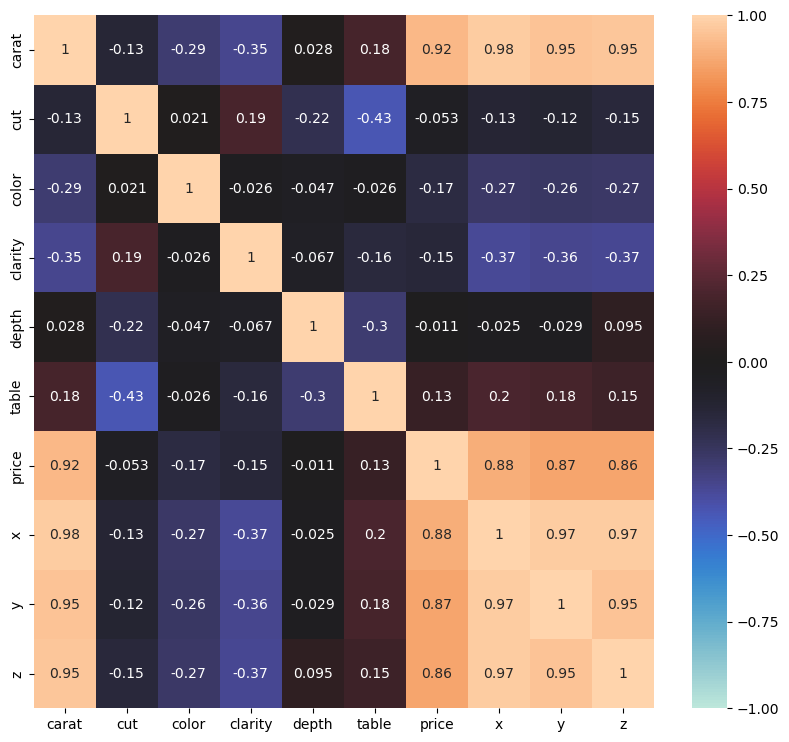
\includegraphics[width=0.5\linewidth]{../Figures/Question-1/datasetCorrHeatmap.png}
   \caption{Feature Pearson Correlation Heatmap}
   \label{fig:corr_hm}
\end{figure}

We will be using the nine features to predict the \texttt{price}. We can begin by 
computing the Pearson correlation matrix heatmap for these features in 
the dataset in Figure 1. The values for correlation for \texttt{price} is given in 
Table 1(a). We see that, unsurprisingly, there is a massive collection of high 
correlation squares at the bottom right. These indicate high Pearson 
correlation coefficient between \texttt{price} and \texttt{x}, \texttt{y}, 
\ texttt{z}. This suggests that 

%%%%%%%%%%%%%%%%%%%%%%%%%%%%%%%%%%%%%%%%%%%%%%%%%%%%%%%%%%%%%%%%%%%%%%%%%%%%%%%%

\begin{table}[H]
\begin{subtable}[H]{0.45\textwidth}
    \begin{tabular}{c l}
        \hline
        \multicolumn{2}{c}{Correlation}         \\
        \hline 
    \texttt{carat}   & 0.9215914337868304    \\
    \texttt{cut}     & -0.05349263851362828  \\
    \texttt{color}   & -0.1725093772499559   \\
    \texttt{clarity} & -0.14680175361025616  \\
    \texttt{depth}   & -0.010647725608533299 \\
    \texttt{table}   & 0.12713358133531918   \\
    \texttt{x}       & 0.8844357793744166    \\
    \texttt{y}       & 0.865421694764742     \\
    \texttt{z}       & 0.861250266123968    \\
    \end{tabular}
    \caption{Price}
    \end{subtable}
    \begin{subtable}[H]{0.45\textwidth}
        \begin{tabular}{c l}
            \hline
            \multicolumn{2}{c}{Correlation}         \\
            \hline 
        \texttt{carat}   & 0.7694571626172851    \\
        \texttt{cut}     & 0.00542011950342582   \\
        \texttt{color}   & -0.011980043670033661 \\
        \texttt{clarity} & 0.04512538515850012   \\
        \texttt{depth}   & -0.03572374489729493  \\
        \texttt{table}   & 0.08458507638109278   \\
        \texttt{x}       & 0.7873455524189906    \\
        \texttt{y}       & 0.7717301198408058    \\
        \texttt{z}       & 0.7655421629234554   \\
    
        \end{tabular}
        \caption{Price per Carart}
    \end{subtable}
    \caption{Pearson Correlation Coefficients}
\end{table}
%%%%%%%%%%%%%%%%%%%%%%%%%%%%%%%%%%%%%%%%%%%%%%%%%%%%%%%%%%%%%%%%%%%%%%%%%%%%%%%%




\end{document}

